%TODO - hodai: fix Automata vs Automaton and axis vs axes

\documentclass{sig-alternate-ipsn13}

\usepackage{array}
\usepackage{url}
\usepackage{cite}
\usepackage{subfigure}
\usepackage{float}
\usepackage{pdfpages}

%%%%%%%% Package for source-code listing %%%%%%%%%%%%
\usepackage{textcomp,listings}
\definecolor{javared}{rgb}{0.6,0,0} % for strings
\definecolor{javagreen}{rgb}{0.25,0.5,0.35} % comments
\definecolor{javapurple}{rgb}{0.5,0,0.35} % keywords 

\lstset{
	language=Java,
	frame=lines,
	captionpos=b,
	basicstyle=\color{blue!30!black!90!green} \ttfamily, % print whole listing small
	keywordstyle=\color{javapurple}\bfseries,%\underbar, underlined bold black keywords
	identifierstyle=, % nothing happens
	commentstyle=\color{javagreen}, % white comments
	stringstyle=\color{javared}, % type for strings
	showstringspaces=false, % no special string spaces
	mathescape=true, % allow math typesetting in listings
	upquote=true,
}
%%%%%%%% Package for source-code listing %%%%%%%%%%%%


%%%%%%%% Packages for drawing diagrams %%%%%%%%%%%%%%%
\usepackage{tikz,ifthen}
\usetikzlibrary{arrows,automata,positioning }
\tikzstyle{block}=[rectangle, draw, thin, inner sep=3pt, text centered, 
%drop shadow, 
fill=orange!20!yellow!20] 
\tikzstyle{pre}=[<-,shorten <=1pt,>=stealth']
\tikzstyle{post}=[->,shorten >=1pt,>=stealth'] 
\tikzstyle{bi}=[<->,shorten >=1pt,shorten <=1pt,>=stealth'] 
\tikzstyle{every initial by arrow}=[initial text={},initial distance=1em,post]
%\tikzstyle{every state}=[minimum size=0.4cm,drop shadow,fill=orange!20!yellow!20]
\tikzstyle{transition}= [post,shorten >=1pt,node distance=2cm, inner sep=2pt,bend angle=20]
\tikzstyle{box}=[rectangle,draw=black, thick, inner sep=3pt, text centered]
%%%%%%%% Package for drawing diagrams %%%%%%%%%%%%%%%

\newcommand\esti{{\lstinline'estimate'}}
\newcommand\simu{{\lstinline'simulate'}}
\renewcommand\j[1]{{\lstinline'#1'}}

\usepackage[english]{babel}
\usepackage{graphicx}
\usepackage{amssymb}
%\usepackage{caption}
%\usepackage{MnSymbol}

\RequirePackage{pgf,pgffor}

\usepackage[mathcal]{euscript}
%%% END LaTeX-Packages ----------------------------------

%\usepackage{amsthm}
\usepackage{setspace}
\newcommand\tuple[1]{\langle #1 \rangle}

\newcommand\sSF[1]{$\Diamond$\footnote{SF: \sout{#1}}}
\newcommand\sIL[1]{$\Diamond$\footnote{IL: \sout{#1}}}
\newcommand\sMA[1]{$\Diamond$\footnote{MA: \sout{#1}}}
\newcommand\sGW[1]{$\Diamond$\footnote{GW: \sout{#1}}}


\newcommand\SF[1]{$\bigstar$\footnote{SF: #1}}
\newcommand\IL[1]{$\bigstar$\footnote{IL: #1}}
\newcommand\MA[1]{$\bigstar$\footnote{MA: #1}}
\newcommand\GW[1]{$\bigstar$\footnote{GW: #1}}

\newcommand\R{{\mathbb R}}
\newcommand\N{{\mathbb N}}
\newcommand\must{$\mathtt{must}$}
\newcommand\bad{$\mathtt{bad}$}
\newcommand\code[1]{{\small \sf #1}}

%%% LaTeX definitions -----------------------------------------
\newtheorem{thm}{Theorem}
\newtheorem{dfn}[thm]{Definition}
\newtheorem{con}[thm]{Construction}
\newtheorem{prop}[thm]{Proposition}
\newtheorem{claim}[thm]{Claim}
\newtheorem{remark}{Remark}

\DeclareMathOperator*{\guard}{guard}
\DeclareMathOperator*{\sensor}{sen}
\DeclareMathOperator*{\actuator}{act}

\newcommand{\mathsym}[1]{{}}
\newcommand{\unicode}[1]{{}}

\newcommand{\M}{{\mathcal{M}}}
%%% END own LaTeX definitions ---------------------------


\begin{document}

\title{Reactive Scheduling of Computational \\ Resources in Control Systems}
%
% You need the command \numberofauthors to handle the 'placement
% and alignment' of the authors beneath the title.
%
% For aesthetic reasons, we recommend 'three authors at a time'
% i.e. three 'name/affiliation blocks' be placed beneath the title.
%
% NOTE: You are NOT restricted in how many 'rows' of
% "name/affiliations" may appear. We just ask that you restrict
% the number of 'columns' to three.
%
% Because of the available 'opening page real-estate'
% we ask you to refrain from putting more than six authors
% (two rows with three columns) beneath the article title.
% More than six makes the first-page appear very cluttered indeed.
%
% Use the \alignauthor commands to handle the names
% and affiliations for an 'aesthetic maximum' of six authors.
% Add names, affiliations, addresses for
% the seventh etc. author(s) as the argument for the
% \additionalauthors command.
% These 'additional authors' will be output/set for you
% without further effort on your part as the last section in
% the body of your article BEFORE References or any Appendices.

\numberofauthors{2} %  in this sample file, there are a *total*
% of EIGHT authors. SIX appear on the 'first-page' (for formatting
% reasons) and the remaining two appear in the \additionalauthors section.
%
\author{
% You can go ahead and credit any number of authors here,
% e.g. one 'row of three' or two rows (consisting of one row of three
% and a second row of one, two or three).
%
% The command \alignauthor (no curly braces needed) should
% precede each author name, affiliation/snail-mail address and
% e-mail address. Additionally, tag each line of
% affiliation/address with \affaddr, and tag the
% e-mail address with \email.
%
% 1st. author
    \alignauthor Gera Weiss\\
       \affaddr{Ben-Gurion University}\\
       \affaddr{Beer-Sheva, Israel}\\
       \email{geraw@cs.bgu.ac.il}
% 2th. author
    \alignauthor Hodai Goldman\\
        \affaddr{Ben-Gurion University}\\
        \affaddr{Beer-Sheva, Israel}\\
        \email{hodaig@cs.bgu.ac.il}
}

\maketitle
\begin{abstract}
We present an approach to scheduling computations in software control systems. The proposed scheduling mechanism is reactive in the sense that it changes the schedule dynamically based on physical conditions. Our proposal is an extension of the automata based scheduling approach with an addition of guards to transitions that allow for reactive specifications. We develop a methodology for using Klman filters to provide data that guides these automata and demonstrate the combined approach in simulations and with a case study of stabilizing a quadcopter in front of a window.    
\end{abstract}

\section{Introduction}
Cyber-physical systems (CPS) technologies of integrating software and control are at the heart of many critical applications (c.f.~\cite{lee2008cyber}). 
These technologies aim at handling issues that emerge when the integration of software and hardware brakes the traditional abstraction layers: when researchers and practitioners are required to consider a unified view that includes both software and hardware. An example of such an issue is the challenge of dynamic assignment of computational resources to software based controllers discussed in, e.g.,~\cite{arzen2000introduction,tabuada2007event,weiss2007automata}. While the computation burden required by the control loops can be ignored in many situations, this is not always the case. A main motivating example studied in this paper is vision based control, where computer vision algorithms acquire state information to be used in a feedback loop (c.f.~\cite{das2002vision,shakernia1999landing,Efraim2017}). Unlike conventional sensors such as accelerometers, gyros, compasses, etc., a visual sensor requires significant processing of the acquired image to prepare the state information for feedback. Since typical cyber-physical application, such as robot control, consist of many control loops, responsible for different aspects of the system, that run simultaneously and share the same computational resources, the computer vision algorithms cannot always be invoked in full power. Alternatively, we propose in this paper a mechanism to dynamically trade CPU consumption vs. measurement accuracy so that data acquisition algorithms run in full power only when the control loop requires accurate data. 

A main challenge in forming mechanisms for the integration of software and control lies in the design of efficient interfaces for integrating the engineering diciplines involved (c.f.~\cite{weiss2007automata}). Components with clearly specified APIs, such as Java library classes, allow designers to build
complex systems effectively in many application domains.  The key to such modular development is
that an individual component can be designed, analyzed, and tested without the knowledge of other
components or the underlying computing platform. When the system contains components with
real-time requirements, the notion of an interface must include the requirements regarding
resources, and existing programming languages provide little support for this.  Consequently,
current development of real-time embedded software requires significant low-level manual effort for
debugging and component assembly (cf.  \cite{Lee00,IEEE03,HS06}).  This has motivated many
researchers to develop compositional approaches and interface notions for real-time scheduling (cf.
\cite{RS01,dH01,MF01,CAHS03,SL08,SLBS04,TWS06,DBLP:conf/lctrts/AuerbachBIKRRT07}).


In this paper we present an approach, a proof-of-concept implementation, and a case-study in scheduling computations in embedded control systems. Our approach is based on the automata based scheduling approach, suggested in~\cite{WA07,RTComposer,AW08}, where automata are proposed as interfaces that allow the dynamicity and efficiency of desktop operating systems with the predictability of real-time operating systems. The approach allows for components to specify the CPU resources that they need in a way that gives an application agnostic scheduler the freedom to choose schedules at run-time such that the needs of all the components are met, even of components that were added only at run-time.  The main contributions of this paper relative to the earlier work in this direction is:
(1) We propose an extension of the automata based scheduling frame work that allows to direct the schedule based on the state of the controllers; (2) We propose a technique, based on the theory of Kalman Filters, for designing reactively scheduled controllers; (3) We report on our experience with improving the performance of real-time a vision-based control system (a quadrotor that stabilizes itself in front of a window).

\section{The proposed approach}
\label{sec:architecture}

As proposed in earlier work on automata based scheduling (cf.~\cite{WA07,RTComposer,AW08}) we aim at a development process where a system is built as a composition of a set of components where each component is a aoftware module ( set of procedures) accompanied with an automaton. Our addition here is that we allow the automata to be guarded, i.e., each automaton acts as a specification of a reactive system that tells the scheduler which functions of a component it may run in each slot depending on the dynamic state of the controllers. A second addition is that we have implemented the approach as an enhancement of the internal scheduler of  the Auto Pilot Mega (APM) open source unmanned vehicle autopilot software suite. A third contribution of the paper is a proposal of a specific way to use the automata based scheduling framework with a Kalman filter. We elaborate on each of these in the following subsections:

\subsection{Guarded Automata as Interfaces for Control and Scheduling}
As our goal is to allow dynamic selection of the computation load in the feedback loops based on the states of the systems, we start with a general software architecture in which each component (implementation os a specific loop) is represented by a code module (in our case, a class in C++) and an automaton that specifies when to invoke its methods. The transition relation of the automaton depends, in addition to the current state, also on a real number produced by the estimator of the feedback loop (we experimented with different options for this number, as discussed below).

The motivations of using automata as described above are: (1) automata allow for a rich specification language; (2) it is easy to construct that obey the specification with negligible computational burden; (3) automata theory gives a solid framework for composing the specifications of competing requirements for analysis and for schedule synthesis. 

In this paper we focus on the first two motivations in the above list. The third is discussed in details in earlier paper on automata based scheduling (cf.~\cite{WA07,RTComposer,AW08}) and is the focus of another paper that we are preparing where we describe some analysis techniques we have developed for guarded automata.   

\subsection{Implementation in an Auto Pilot Software}
As our main case study is in flight control, we chose the ArduPilot Mega
(APM) platform for experiments. To this end, we implemented a basic automata based scheduler for this platform. The task scheduling specification in APM consist of a table as shown in Figure~\ref{fig:apm-scheduler}. This table is easy to maintain and to use, but it is used under an assumption that there is enough CPU power to run all the tasks can run in the specified frequencies. APM does contain a mechanism to handle overruns, by moving tasks to the next window when there is not enough time to run them now, but the system is designed under the assumption that only happen in rare situations.

We replaced this table with automata that specify when to run the tasks. Note that automata allow for specifying the requirements that the table represents, using simple circular automata without guards. Note also, that automata can model more advanced constraints with very little addition to the complexity of the scheduler, as we will demonstrate later in the paper. 

\begin{figure}
	\scriptsize
	\begin{lstlisting}
/*
  scheduler table - all regular tasks apart from
  the fast_loop() should be listed here, along 
  with how often they should be called (in 10ms 
  units) and the maximum time they are expected 
  to take (in microseconds)
*/
static const AP_Scheduler::Task 
     scheduler_tasks[] PROGMEM = {
	{ update_GPS,            2,     900 },
	{ update_nav_mode,       1,     400 },
	{ medium_loop,           2,     700 },
	{ update_altitude,      10,    1000 },
	{ fifty_hz_loop,         2,     950 },
	{ run_nav_updates,      10,     800 },
	{ slow_loop,            10,     500 },
	{ gcs_check_input,       2,     700 },
	{ gcs_send_heartbeat,  100,     700 },
	{ gcs_data_stream_send,  2,    1500 },
	{ gcs_send_deferred,     2,    1200 },
	{ compass_accumulate,    2,     700 },
	{ barometer_accumulate,  2,     900 },
	{ super_slow_loop,     100,    1100 },
	{ perf_update,        1000,     500 }
};
	\end{lstlisting}
	\caption{APM scheduling specification}
	\label{fig:apm-scheduler} 
\end{figure}


\subsection{Integration With a Kalman Filter}
The third layer of the approach we propose is the observation that a standard Kalman filter produces information that can be used to guide the automata of the components. 

As we will elaborate in the description of the simulations and of the case study below, we propose to schedule the functions that implement algorithms for sensing and for actuation based on the variance of the estimation that a Kalman filter provides. 



%\section{An example driven description of the proposed approach}
\section{A demonstration of the approach in simulation}

Our approach for using automata for scheduling resources in software based controllers is based on the observation that in most systems the computational load is in the implementation of the sensors and of the actuators, not in the implementation of the controllers that usually consist of quick arithmetic manipulation of a small amount of variables. We therefore focus our attention on allowing a trade-off between CPU usage of sensors and actuators and their accuracy. In this paper, as a main motivating example, we focus on the case of visual sensors that employ image processing algorithms.

As said in Section~\ref{sec:architecture}, we propose to implement the resource scheduling decisions using automata that control which procedures are invoked in the control loops. More specifically, for sensors or actuators that require heavy computations, such as vision based sensors, we propose that the software engineers develop several modes of sensing, each consumes a different amount of CPU and provides a different level of accuracy. 

Formally, we assume that the system is given as a Linear Time Invariant system, as depicted in Figure~\ref{fig:simulink}. The inaccuracies of the sensors and of the actuators are modeled as additive Gaussian noise. We assume that each sensor can be operated in a range of modes (more than one), each mode consuming a certain percentage of the CPU and giving a certain variance of the measurement noise.

\begin{figure}%[htbp]
	\centerline{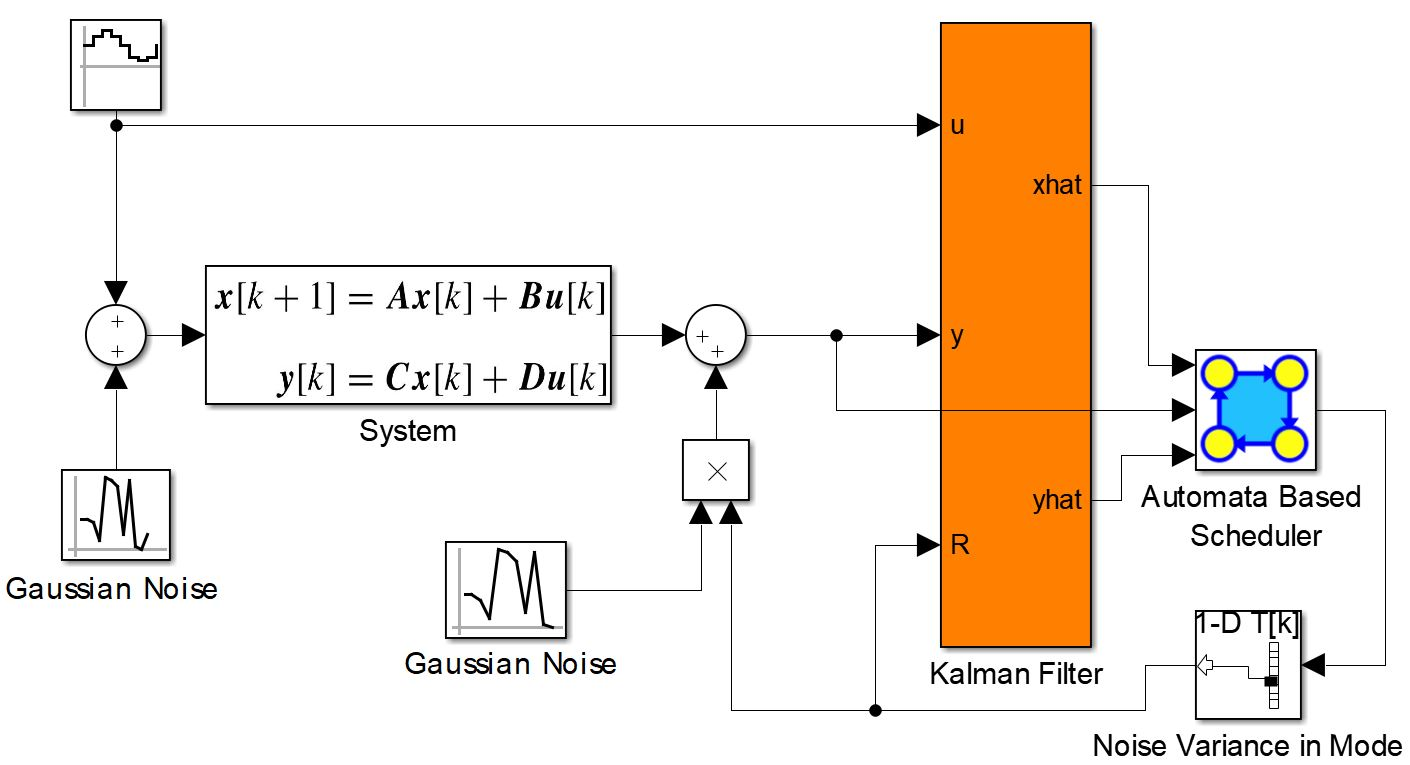
\includegraphics[width=85mm]{SimulinkModel.jpg}}
	\caption{A Simulink model demonstrating the proposed approach.}
	\label{fig:simulink}
\end{figure}

The scheduling of the modes is governed by the automata based scheduler as depicted in Figure~\ref{fig:simulink}. We propose to use a standard Kalman filter for the purpose. The filter gets as input the actuations and the measurements (the sum of the output and the noise) and also the variance of the measurement noise, which we assume is a function of the sensor mode chosen by the scheduler. The output of the Kalman filter and the measurement are fed to the scheduler (in addition to, possibly, sending them to the controller) that uses them for deciding the next mode of the sensor. In the Simulink model depicted in Figure~\ref{fig:simulink}, the scheduler feeds the variance of the disturbance to the Kalman filter and to the block that multiplies the noise by the variance (the product of a white noise with unit variance and a constant $C$ yields a normally distributed noise with variance $C$).

We ran the model depicted in Figure~\ref{fig:simulink} with the linear time invariant system:
\begin{eqnarray*}
x(k+1) &=& \begin{pmatrix}
	1.3  & -0.5  & 0.1 \\
	1    & 0     & 0 \\
	0    & 1     & 0
\end{pmatrix}x(k)+ 
\begin{pmatrix}
-0.4 \\
0.6\\
0.5\end{pmatrix} u(k) \\
y(k)&=& \begin{pmatrix}1 & 0 &0\end{pmatrix}x(k)
\end{eqnarray*}
taken from \url{https://www.mathworks.com/help/control/examples/kalman-filter-design.html}. As seen in Figure~\ref{fig:simulink}, we injected a sinusoidal input (with $amplitude=bias=frequence=1$) to this system. 
The actuation noise, depicted on the left, is with a unit variance. 

The `Automata Based Scheduler' block is designed to set the variance of the sensing noise dynamically to be either $0.25$ or $1$ at each step of the simulation. This models a sensor that has two modes of operation: a mode with high accuracy that produces noise with low variance and a mode with low accuracy that produces errors with higher variance. We assume, for the performance measurements presented below, that the CPU consumption of each mode is $\%CPU=1.1-errVar$, where $errVar$ is the variance of measurement error in the mode.

We ran this models with three versions of the `Automata Based Scheduler' block. The first version, called `High' in Table~\ref{tbl:sim-results}, is where the block acts simply as the constant $1$, ignoring its inputs altogether. Similarly, the term `Low' in the table refers to an implementation where the block is the constant $0.25$. These two implementations model the constant schedules, where the sensor is operated in one mode along the whole execution. These two schedules are compared to a third implementation, called 'Automaton' in the table, where the block implements the schedule given by the automaton:
%TODO - hodai say: you forgot  to put the automaton inside figure??
%TODO-Gera say: No. I don't see a reason to put it in a figure :-)
\begin{center}
\begin{tikzpicture}[->,>=stealth',shorten >=1pt,auto,node distance=6cm,
semithick]

\node[initial,state] (A)                 {$1$};
\node[state]         (B) [right of=A]    {$0.2$};

\path (A) edge [bend left]             node {$|y-\hat{y}|\geq1$} (B)
      (A) edge [loop below] node {$|y-\hat{y}|<1$} (A);
      
\path (B) edge [bend left]             node {$|y-\hat{y}|\leq 1/2$} (A)
      (B) edge [loop above] node {$|y-\hat{y}|>1/2$} (B);
      
\end{tikzpicture}
\end{center}
where the name of a state defines the variance of the estimation noise when entering it.
%A = [1.1269   -0.4940    0.1129,
%1.0000         0         0,
%0    1.0000         0];
%
%B = [-0.3832
%0.5919
%0.5191];
%
%C = [1 0 0];

\begin{table}
	\centering
	\begin{tabular}{ |  l  | c | c | c | }
		\hline
		&  High & Low & Automaton \\ \hline \hline
		\%CPU                    & 0.85 & 0.1  & 0.46 \\ \hline
		mean of $|x -\hat{x}|$ & 0.97 & 1.24 & 1.08 \\ \hline
	\end{tabular}
	\caption{Simulation results.}
	\label{tbl:sim-results}
\end{table}

The results of the simulation, summarized in Table~\ref{tbl:sim-results}, show, as expected, that the CPU consumption is much lower (0.1) when using the low-quality version of the sensing algorithm and is higher (0.85) when the high-quality version of the sensing algorithm is used. The performance of the estimation in terms of the mean distance between $x$ and $\hat x$ better with the high-quality version (0.97) than it is with the low-quality version (1.24).
More interestingly, we can see that the experiment with the automaton that switches between the two sensor modes yields performance that is close to the performance of the high-quality sensing algorithm, using much less CPU. 








%\begin{enumerate}
%    
%    \item \textbf{Controller design:} Based on the separation principle, we propose to design the controller to achieve the control objectives assuming a perfect observation. In practice, this may not be feasible because controller designs such as PID require a system to experiment with. In this case, as demonstrated in the case-study below (see Section~\ref{sec:caseStady}), we propose to work with one of the observation modes. If the system is close to linear, this should result with a near optimal design.
%    
%    \item \textbf{Observers design:} Specification of sensor modes and observers design
%    
%    \item \textbf{Performance analysis:} Now, we can perform some experiments with the different observer modes and analyze transient behaviors. Specifically, as shown in the case study~\ref{sec:caseStady_analysis}, we can measure how long it takes for the error to accumulate after switching to a lesser observation mode and formulate how this error affects the control objectives.
%
%    \item \textbf{Scheduling automata design:} Base on the analysis we can specify the resource scheduling requirements in the form of \textit{specification automaton}. The goal is to design flexible specification that allow dynamic scheduling in order to adapt the environment and the system state, this will improve the system efficient.
%
%\end{enumerate}


%\section{Application to Autonomous Quad-rotor Flying In-Door}
\section{Case Study: Stabilizing a quadrotor in front of a window}
\label{sec:caseStady}
% overview of why we use vision example

%TODO - Window test case problem
The case study we used to test our concept is the development of a controller that stabilizes a quadrotor~\cite{?} in front of a window.
We implement an autonomous controller for that task and evaluated its performance.

The part of the controller that we focused on is the vision based position controller. Specifically, the main controller, that we will describe below, uses a standard low-level angular controller and a simple image processing algorithm that identifies the position of the corners of the window in the image plane\footnote{In the experiment, to simplify the image processing algorithm, we marked the corners of the window with led lights.}. Its goal is to regulate the position of the quadrotor by tilting it. Note that rotations of the quadrotor generate a more-or-less proportional accelerations in a corresponding direction. A main challenge for this controller is that the computer vision algorithm takes significant time to compute relative to the fast control loop. We can decrease computation time by lowering the resolution, but this also increase the measurement noise. We will demonstrate how adaptive scheduling of the resolution can serve for balancing resource consumption vs. control performance.

\subsection{Observer Design}
\label{sec:Observer Design}
We first implemented an observer based on the work of Efraim at al.~\cite{?? Dynamic Image Based Visual Servo Control of Micro Aerial Vehicles Relative to a Window}. The observer gets the positions of the widow corners, enumerated clockwise starting from the top left corner noted by $p_1,p_2,p_3,p_4$, and extract 4 quantities based on the shape and location of the window corners in the image plane: $S_x$ , $s_y$ , $V_d$ and $sz$.
\textbf{center of mass:} $S_x$ and $S_y$ represent the window ``center of mass'' in the image plane along the image $x$ and $y$ axes, respectively. $S_x$ and $S_y$ are normalized to the range of $[-1,1]$.
$S_x$ is used to measure the roll angle of the window center (for stabilize the roll axis), and $S_y$ is used to measure the altitude of the drone (for stabilizing the throttle).
\textbf{Window size:} $sz$ is the sum of the vertical edges of the window, $sz$ is used to measure the distance of the drone from the window and then to regulate the roll angle~\footnote{we use fixed size window and convert $sz$ to distance (in meter in our case) based on this window, in the general case the distance is relative to the window size}.
\textbf{Vertical difference:} $V_d = \frac{y_1-y_4-(y_2-y_3)}{y_1-y_4+(y_2-y_3)}$, were $y_i$ is the vertical position of $p_i$ in the range of $[-1,1]$ (0 is the center of the image) first is used to measure the angular position of the drone in relation to the window ($\theta$), then $\theta$ and $sz$ are used to calculate the horizontal position parallel to the window surface ($x$ position) of the drone (see Figure~\ref{fig:axis}). 

%TODO - hodai say: not sure how to define this note:
\begin{remark}
    We assume that process state ($x$) is governed by the linear~\footnote{we make approximation of our non-linear system by linear difference equation} stochastic difference equation:
    $$x_{k}=Ax_{k-1} + Bu_{k} + w_{k}$$
    And the measurement ($z_k$) at time $k$ is:
    $$z_k=Cx_k+v_k$$
    The random variables $w_k$ and $v_k$ represent the process and measurement noise (respectively).
\end{remark}

After measuring the relative position and yaw attitude, as usual, we add estimator filter to get better state estimation. 
%TODO : check if its realy shown there:
In theory, and s shown in the simulation at Section~\ref{sec:simulation}, we should use Kalman filter estimator for best state estimation, in our case is non-linear system and the process noise distribution is problematic to determine (battery state affects the system dynamics), this with the complexity of kalman filter lead us simplify the kalman filter principles using complementary filter, a simple estimation technique that is often used in the flight control industry.
Complementary filter is actually a steady-state Kalman filter for a certain class of filtering problems~\cite{complementaryVSKalman}.
We use two steps estimator that, (1) \textit{predict} the current state evolved from the previous state using a linearized model of the system ($\hat{x_{k|k-1}}$) and then \textit{update} the prediction with current state measurement from image, noted by $z_k$.
The result estimation (noted by $\hat{x}_{k|k}$) is a complementary filter of the prediction ($\hat{x}_{k|k-1}$) and the measured state ($C^{-1}z_k$):
$ \hat{x}_{k|k} = K \hat{x}_{k|k-1} + (1-K) C^{-1}z_k $ were $K$ is constant approximation of the kalman filter gain ($K_k$).

The image processing have few different operation modes, every mode has different accuracy (shown in Section~\ref{sec:Analysis}).
Similarly to the gain of kalman filter, $K$ represent the ratio between process noise and measurement noise distribution, therefore $K$ is defined separately for each mode to achieve the best estimation in each mode.

\begin{figure}[htbp]
    \centerline{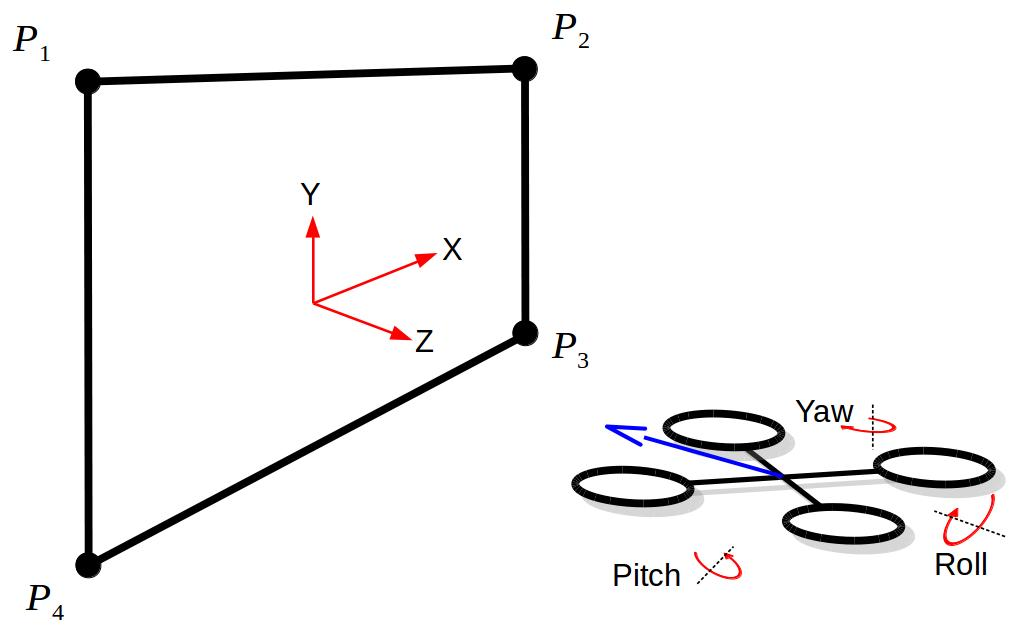
\includegraphics[width=80mm]{axis.jpg}}
    \caption{Description of Coordinate System and Rotation Axis.}
    \label{fig:axis}
\end{figure}


\subsection{Controller Design}

In this experiment, we consider the task of \textit{hovering in front of the window}, the controller objective is to hover parallel to the window (center of $x$ axis) at the altitude of the window within distance of 2 meters in front of the window and face pointed to the center of the window (yaw angle).
We consider this point as the origin and the coordinates are according to Fig.~\ref{fig:axis}.

The controller consist of 4 independent feedback control loops, altitude, yaw angel, pitch and roll.
Pitch and roll controllers composed from, low level attitude controller which his input is the required pitch or roll angel accordingly, and high level position controller which his input is the required distance or $x$ position relative to the window accordingly, the high level controller outputs the required angle (acceleration) to the low level controller as show in Fig.~\ref{fig:controllerStracture}.
All the loops control regulate the position or attitude relative to the window.
The inertial (angular) feedback is generated by the existing \textit{Attitude and heading reference system} (AHRS) library of ArduPilot see Section~\ref{sec:Experiment setup}, and the window related feedback come directly from the observer described in Section~\ref{sec:Observer Design}.

Based on the separation principle, we can use that controller regardless the measurement quality, in practice we implement basic Proportional Integral Derivative (PID~\cite{aastrom2006advanced}) controller and tuned the parameters with the highest resolution observer.

%TODO - Hodai say: I think this figure is un-nesessary.
\begin{figure}[htbp]
    \centerline{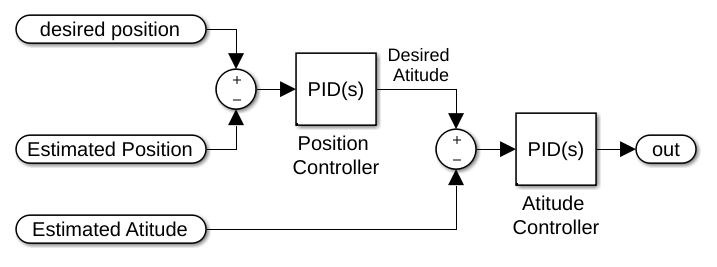
\includegraphics[width=85mm]{two_level_controller.jpg}}
    \caption{Atitude and Position Controller - Two level structure}
    \label{fig:controllerStracture}
\end{figure}


%%%%%%%%%%% Specification Automata %%%%%%%%%%%%%
\subsection{Analysis and Specification Automata}
\label{sec:Analysis}
%As describe in Section~\ref{sec:???}, the image processing have few different operation modes, every mode use different image resolution, better image resolution results in more accurate measurement but consume more processing time, changing operation modes allows us to control the trade off between mesurment quality and processing time as shown in Table~\ref{tab:tradeoff ???}.

The objective of the system is to maintain stable hovering in front of the window. Hence, the performances of the system is measured by the amount of deviation from the center line of the window in the critical axis $x$, meaning, we want to minimize $|x|$ (see Figure~\ref{fig:axis}). Our goal is to achieve maximum performance with minimal amount of processing time. Obviously, both goals can not be achieved together, the task is to set the best trade-off between them. The problem comes from the main consumer of computation resources, the image-based observation tasks.
In this part, we use different observation modes together in order to improve the resource utilization, meaning we use more resources (CPU time) only when it is needed, and this way reduce the overall CPU usage without significantly affect the performance.
In fact, we switch the camera resolution during the flight, the image resolution define the operation mode (see Section~\ref{sec:Observer Design}).
For simplicity, in this work we examine only two modes, \textit{High quality} with resolution of 960p and \textit{Low quality} with resolution of 240p.

Analyzing the test results shown in Table~\ref{tab:results}, we see that High quality observation mode provide mean ($x$) error tolerance of 9.5 \textit{cm}~\footnote{All lengths are measured in Centimeter.}, and with the cost of 30\% CPU usage.
On the other hand, Low quality mode provide worse mean error of co \textit{cm} (three times High quality mode), but cost only 2.1\% CPU usage~\footnote{The CPU usage percentage is the average usage, and is calculates as $\frac{\text{total time spend in image processing}}{\text{total flight time}}$ . }.
In this section we show how defining \textit{adaptive scheduling specification} in order to lower the CPU usage without significant worsening of High quality performances.

%TODO - displacement ($x_{k|k}$) schedulers
First we examine a straight-forward solution based directly on the current position (the $x$ part of $\hat{x}_{k|k}$). Using the simple guard automaton $A_{x}$ presented in Fig.~\ref{fig:test_automata}, we define dynamic observer that choose the operation mode (high or low quality) based on the $x$ part of $\hat{x}_{k|k}$ absolute value, if the drone is closer to the center line of the window, noted by $|x| < T_x$, we consider it as ``safe'' state and go to $L$ mode that use the low quality image.
Similarly, ``BAD'' states are when the drone is far, noted by $|x| > T_x$, then we use High quality image in order to ``fix'' the bad state.
The trash-hold $T_x$ value can be changed to define the desire performances and processing time trade-off.
Results shows good improvement in term of resource utilization (see Section~\ref{sec:results}). 

%TODO - error ($y_{k|k}$) schedulers
\begin{dfn}
\textit{Measurement post-fit residual} $\tilde{y}_{k|k}$, is the difference between the expected measurement ($C \cdot \hat{x}_{k|k}$) and the measured state ($z_k$): $\tilde{y}_{k|k} = |  \hat{x}_{k|k} - z_k |$~\footnote{ Measurement post-fit residual $\tilde{y}_{k|k}$ is also defined by Kalman filter}.
\end{dfn}
From the Low quality experiment graph we can see that $\tilde{y}_{k|k}$ accumulates proportional to the deviation from the center of $x$ axis, we can use $\tilde{y}_{k|k}$ vales to predict high deviation from $x$.
In the second experiments set we used $A_{err}$ Automaton presented in Fig.~\ref{fig:test_automata}, which is similar to $A_x$ but switch states based on $\tilde{y}_{k|k}$ value.
In this case the observer operate in low quality when $\tilde{y}_{k|k} < \alpha_{low}$ (``GOOD'' state), and change to high quality when $\tilde{y}_{k|k} > \alpha_{high}$ (``BAD'' state).
The trash holds values $ \alpha_{low}$ and $ \alpha_{high}$ has determined first from the low and high quality graph and fine tuned by experiments. 
Different $ \alpha_{low}$ and $ \alpha_{high}$ achieve different trade-offs of performances and processing time.
Note, in Section~\ref{sec:results} we show how this dynamic observer do not result significant affect to the performance but reduce by factor of $\frac{1}{2}$ the processing time.









%TODO - continue here

%TODO hodai: complex / agregated schedulers (3 states) - the results shows no improvement I wont to perform new experiments with significant improvement

%TODO - gyro derived?? more suggestions?

%%%%%%%%%%%%%%%%%%%%%%%%%%%%%%%%%%%%%%%%%%%%%%%%%%
%%%%%%%%%%%%%%% automata %%%%%%%%%%%%%%%%%%%%%%%%%
%%%%%%%%%%%%%%%%%%%%%%%%%%%%%%%%%%%%%%%%%%%%%%%%%%
\tikzset{every edge/.append style={font=\small}}
\tikzset{every node/.append style={font=\small}}
\begin{figure}[htbp]
    %\captionsetup{width=0.4\textwidth}
    \centering
    \begin{tabular}{c c}
    
        % by error
        \begin{tikzpicture}[node distance=2.5cm,auto]
            \node (A) [state, accepting] {$\{L\}$};
            \node (B) [state, accepting] [right of=A] {$\{H\}$};
            
            \path[->] (A) edge [loop above] node {$|\tilde{y}_{k|k}| < T_l$} (A);
            \path[->] (A) edge [bend left] node {$|\tilde{y}_{k|k}| > T_l$} (B);
            \path[->] (B) edge [bend left] node {$|\tilde{y}_{k|k}| < T_h$} (A);
            \path[->] (B) edge [loop above] node {$|\tilde{y}_{k|k}| > T_h$} (B);
            %\path[->] (B) edge [bend left] node {$s_{0.7} \wedge est_1$} (A);
        \end{tikzpicture}

        &
        
        % by displacement (|x|)
        \begin{tikzpicture}[node distance=2.5cm,auto]
            \node (A) [state, accepting] {$\{L\}$};
            \node (B) [state, accepting] [right of=A] {$\{H\}$};
            
            \path[->] (A) edge [loop above] node {$|x| < T_x$} (A);
            \path[->] (A) edge [bend left] node {$|x| > T_x$} (B);
            \path[->] (B) edge [bend left] node {$|x| < T_x$} (A);
            \path[->] (B) edge [loop above] node {$|x| > T_x$} (B);
            %\path[->] (B) edge [bend left] node {$s_{0.7} \wedge est_1$} (A);
        \end{tikzpicture}
        
        \\
        \LARGE{$A_{err}$} & \LARGE $A_x$ \\[10pt]
        \hline
        
        % 3 state
        \multicolumn{2}{c}{
        \begin{tikzpicture}[node distance=3.5cm,auto]
            \node (A) [state, accepting] {$\{L\}$};
            \node (B) [state, accepting] [right of=A] {$\{L\}$};
            \node (C) [state, accepting] [right of=B] {$\{H\}$};
            
            \path[->] (A) edge [loop below] node {$|x| < T_x$} (A);
            \path[->] (A) edge [bend left] node {$|x| > T_x$} (B);
            \path[->] (B) edge [bend left, above] node {$|x| < T_x$} (A);
            \path[->] (B) edge [loop below] node {$|x| > T_x \wedge |\tilde{y}_{k|k}| < T_l$} (B);
            
            \path[->] (B) edge [bend left] node {$|x| > T_x \wedge |\tilde{y}_{k|k}| < T_l$} (C);
            \path[->] (C) edge [bend left, above] node {$ |\tilde{y}_{k|k}| < T_h$} (B);
            \path[->] (C) edge [loop below] node {$ |\tilde{y}_{k|k}| > T_h$} (C);
            %\path[->] (B) edge [bend left] node {$s_{0.7} \wedge est_1$} (A);
        \end{tikzpicture}
        }
        
        \\ 
        \multicolumn{2}{c}{\LARGE $A_{comp1}$}\\[10pt]
        \hline
        
        % 4 state
        %TODO - Hodai say: this is non-deterministic automata for sipmlicity
        \multicolumn{2}{c}{
            \begin{tikzpicture}[node distance=3.5cm,auto]
            \node (A) [state, accepting] {$\{L\}$};
            \node (B) [state, accepting] [right of=A] {$\{L\}$};
            \node (C) [state, accepting] [right of=B] {$\{H\}$};
            \node (D) [state, accepting] [below=1cm of B] {$\{H\}$};

            \path[->] (A) edge [loop below] node {$|x| < T_x1$} (A);
            \path[->] (A) edge [bend left] node {$|x| > T_x1$} (B);
            \path[->] (B) edge [bend left, above] node {$|x| < T_x$} (A);
            
            \path[->] (B) edge [loop above] node {$else$} (B);
            
            \path[->] (B) edge [bend left] node {$|T_{x2}| > T_x$} (C);
            \path[->] (C) edge [bend left, above] node {$|T_{x2}| < T_x$} (B);
            \path[->] (C) edge [loop below] node {$|T_{x2}| > T_x$} (C);
            
            \path[->] (B) edge [bend left] node {$|\tilde{y}_{k|k}| > T_l$} (D);
            \path[->] (D) edge [bend left] node {$|\tilde{y}_{k|k}| < T_h$} (B);
            \path[->] (D) edge [loop left] node {$|\tilde{y}_{k|k}| > T_h$} (D);
            \end{tikzpicture}
        }
        \\
        \multicolumn{2}{c}{\LARGE $A_{comp2}$}\\
        
        
    \end{tabular}
    
    \caption{The main Automata we used for describing the specifications in the experiments. 
        \newline $A_{err}$ uses the \textit{measurement post-fit residual} ($\tilde{y}_{k|k}$), if $|\tilde{y}_{k|k}|$ is too small then next iteration will use small resolution image ($L$), and if too large the high resolution will be used, $T_l$ and $T_h$ are the transition trash-holds.
        \newline $A_x$ operate similar to $A_{err}$ but uses the current position (the $x$ part of $\hat{x}_{k|k}$) instead $\tilde{y}_{k|k}$, with the trash-hold $T_x$.
        \newline $A_{comp1}$ and $A_{comp2}$ are the results of composing the $A_{err}$ and $A_x$ ideas.}
    
    \label{fig:test_automata}
\end{figure}

%%%%%%%%%%% results %%%%%%%%%%%%%
\subsection{Results}
\label{sec:results}
TODO - graphs and tables

all statistics are taken from real indoor flights of 1-2 minutes


\begin{table}[htbp]
    \caption{Test Results}
    \begin{center}
        \begin{tabular}{m{8em} |  m{4em} m{5em} m{5em}}
        %\begin{tabular}{m{6em} |  c c c}
            \hline
            %\textbf{Observer}& CPU usage (\%)  & Mean displacement ($x$ axis) & Max displacement ($x$ axis)\\
            \textbf{Schedule}& \textbf{\% CPU}  & \textbf{mean(|$x$|) (cm)} & \textbf{max(|$x$|) (cm)}\\
            %\cline{2-3} 
            \hline
            Only High & 30.9\% & 9.5 & 31.2 \\
            \hline
            Only Low & 2.1\% & 30.0 & 70.9 \\
            \hline
            $A_{x}$ \newline ($T_x=10$) & 16.6\% & 10.9 & 42.5 \\
            \hline
            $A_{x}$ \newline ($T_x=20$)  & 14.0\% & 14.1 & \textbf{32.1} \\
            \hline
            $A_{x}$ \newline ($T_x=30$)  & 8.9\% & 17.4 & \textbf{48.4} \\
            \hline
            $A_{err}$ \newline ($T_l=10 , T_h=20$) & 10.3\% & 14.9 & 43.2 \\
            \hline
            $A_{err}$ \newline ($T_l=10$ , $T_h=15$) & 11.7\% & 11.3 & 36.3 \\
            \hline
            $A_{comp1}$ \newline ($T_x=10$ , $T_l=10$ , $T_h=15$)  & 8.8\% & 12.9 & 32.1 \\
            \hline
            $A_{comp2}$ \newline ($T_{x1}=10$ , $T_{x2}=30$ , $T_l=10$ , $T_h=15$)   & 10.4\% & 12.7 & 36.6 \\
            \hline
            
        \end{tabular}
        \label{tab:results}
    \end{center}
\end{table}

\section{Experiment setup}
\label{sec:Experiment setup}

In order to perform the experiments we used of-the-shelf quad rotor with \textit{navio2}~\cite{navio} and \textit{Raspberry pi}~\cite{raspberry} flight controller that runs a modified \textit{ArduPilotMega-arducopter}~\cite{APM} software.
\textit{Navio2} is extension board (shield) for the \textit{Raspberry pi}~\cite{raspberry} platform, it provides the nessesary interfaces such as remote control inputs and motors output, and it's equipped with 3-axes gyroscop and accelerometer MEMS sensors~\cite{MEMS}.
%cammera
We used the standard raspberry pi camera. % and modified driver for eficient recording in 

%the window

%TODO - natnet
%TODO - vision search algorithem??

\section{Conclusions}
Conclusion goes here.


%ACKNOWLEDGMENTS are optional
\section*{Acknowledgments}
Acknowledgement goes here.


%
% The following two commands are all you need in the
% initial runs of your .tex file to
% produce the bibliography for the citations in your paper.
\bibliographystyle{abbrv}
\bibliography{reactive_scheduler}  % reactive_scheduler.bib is the name of the Bibliography in this case
% You must have a proper ".bib" file
%  and remember to run:
% latex bibtex latex latex
% to resolve all references
%
% ACM needs 'a single self-contained file'!
%
%APPENDICES are optional
%\balancecolumns
\appendix
%Appendix A

Appendix goes here.

% That's all folks!
\end{document}
